%% LyX 2.2.1 created this file.  For more info, see http://www.lyx.org/.
%% Do not edit unless you really know what you are doing.
\documentclass[english]{article}
\usepackage[T1]{fontenc}
\usepackage[latin9]{inputenc}
\usepackage[a4paper]{geometry}
\usepackage{amsmath}
\geometry{verbose,tmargin=0.5cm,bmargin=0.5cm,lmargin=0.5cm,rmargin=0.5cm}
\usepackage{graphicx}
%\usepackage[chapter]{algorithm}
\usepackage{algorithmic}

\usepackage{array}
\usepackage{graphicx}
\usepackage{multirow}
\usepackage{tikz}

\usepackage{tabularx}
\usepackage{colortbl}
\usepackage{hhline}
\usetikzlibrary{positioning}

\newcommand\MyBox[2]{
  \fbox{\lower0.75cm
    \vbox to 1.7cm{\vfil
      \hbox to 1.7cm{\hfil\parbox{1.4cm}{#1\\#2}\hfil}
      \vfil}%
  }%
}

\DeclareMathOperator*{\argmin}{\arg\!\min}
\DeclareMathOperator*{\argmax}{\arg\!\max}

\makeatletter

%%%%%%%%%%%%%%%%%%%%%%%%%%%%%% LyX specific LaTeX commands.
%% Because html converters don't know tabularnewline
\providecommand{\tabularnewline}{\\}

\makeatother

\usepackage{babel}
\begin{document}

\title{Machine Learning for Computer Vision (EE5177) \\ Programming Assignment 1 : Fitting Probability Distribution to Data \\ Problem \#2}

\author{Akshit Kumar \\ \emph{EE14B127}}

\date{7th February 2017}

\maketitle
\tableofcontents{}

\section{Problem}
We are given a data set consisting of face and non-face images. The task is to classify a new image as a face or a non face.
\subsection{Goal}
For a given test data, we are required to classify the test data to belong to either a face class or a non face class.
\subsection{Challenges}
Learning a model and doing classification on all 784 dimensions (28x28 greyscale images) is computationally expensive.
\subsection{Approach}
To classify a test data to either class of faces or non faces, we make use of Generative Classification Technique by learning the class conditional probability distributions for the face class and non face class. We train the data to fit Multivariate Normal Distribution for face and non face models using Maximum Likelihood Estimation. Depending on which model gives a better loglikelihood score, we classify the test data into the respective class.
\newline 
To handle the computational infeasibility, we use Principal Component Analysis (PCA) for dimensionality reduction to say some $K$ dimensions ($K$ < 784). To do this, we do eigen value decomposition of the covariance matrix of the training data then order the eigen values from highest to lowest. Now we select the eigen vectors corresponding to the top $K$ eigen values and project the data along these selected eigen vectors which give project the data along the plnae of the highest variance giving the final dimension reduced data. For the test data also, eigen vectors of the corresponding training data are used for reduction. 
\newline
\emph{Note : In this implementation, I used the eigen vectors of the face training data to project all my other train and test data sets to that of the eigen vectors of the face.}
\newline
For getting the best model to choose from, the training set of faces and non faces is divided into different sets and different models are learnt on these training sets of different sizes. The classification results of these models are plotted and the model giving the highest classification accuracy is used.
\newline
We then visualise the likelihood score given by the best model to the test data sets and decide threshold for using the face model alone versus non face model alone but plotting the ROC plots.

\section{Results}
\subsection{Classification Accuracy}
To find the best model in terms of number of faces and non faces, we plot the classification accuracy($A$)which is defined as 
$$ A = \dfrac{tp + tn}{tp + tn + fn + fp} $$ where the confusion matrix is defined as follows:
\newline
$$
\begin{tabularx}{.7\textwidth}{&gt;{\bfseries}c|c c c |}
 & Faces & Non Faces \\
\hhline{----}
Faces & True Positive ($tp$) \cellcolor[gray]{.8}& False Negative($fn$)   \\
Non Faces & False Positive ($fp$) & True Negative ($tn$) \cellcolor[gray]{.8} \\
\hhline{~---}
\end{tabularx}
$$
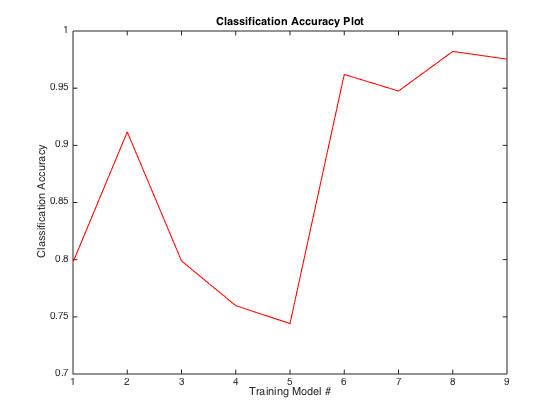
\includegraphics[scale=0.6]{plot_classification_accuracy}
\newline
From this plot we see that the last model (\# of faces = 600 and \# of non faces = 400) gives the best classification accuracy amongst all the models.
\subsection{Visualization of Loglikelihood Scores}
Given that the best model according to the classication accuracy plot is model \#9. We visualise the loglikehood scores given by this model for faces and non faces data set.
\newline
\subsubsection{Loglikelihood Scores On Faces Test Set}
For the model learnt on the training set of faces and non-faces and then tested on face test sets, gives the following plot for loglikelihood scores.
\newline
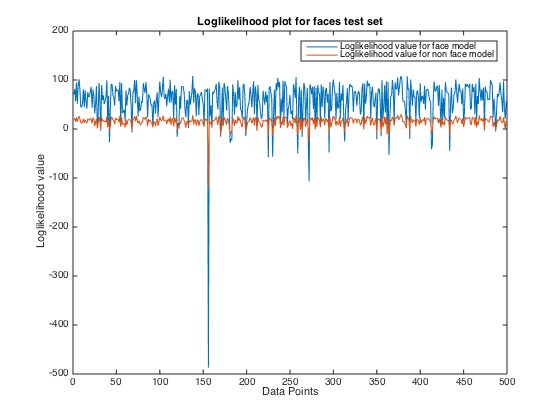
\includegraphics[scale=0.6]{plot_loglikelihood_face}
\newline
To get the threshold for, we set the lower threshold to -50 and increase the threshold to +50 in steps of +1.
\newline 
\subsubsection{Loglikelihood Scores On Non Faces Test Set}
For the model learnt on the training set of faces and non faces and then tested non-face test sets, gives the following plot for loglikelihood scores.
\newline
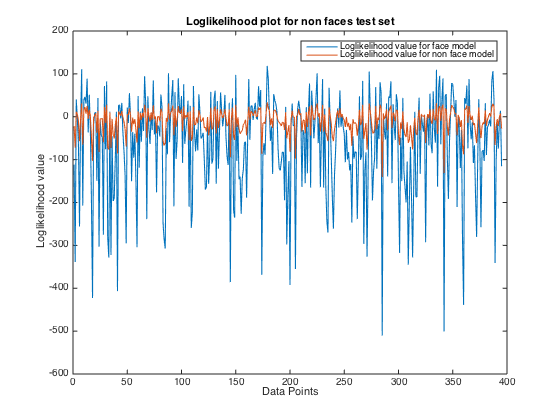
\includegraphics[scale=0.6]{plot_loglikelihood_non_face}
\newline
To get the threshold for, we set the lower threshold to -100 and increase the threshold to +100 in steps of +1.
\subsection{ROC Curve Plots for Face and Non-Face Model}
By iterating through the different values of the threshold, we get different $tp$ and $tn$ and hence we plot the True Positive Rate (TPR) vs False Positive Rate (FPR) which is defined as follows :
$$ TPR = \dfrac{tp}{tp + fn} $$
$$ FPR = \dfrac{fp}{fp + tn} $$
\subsubsection{ROC curve using face model as predictor}
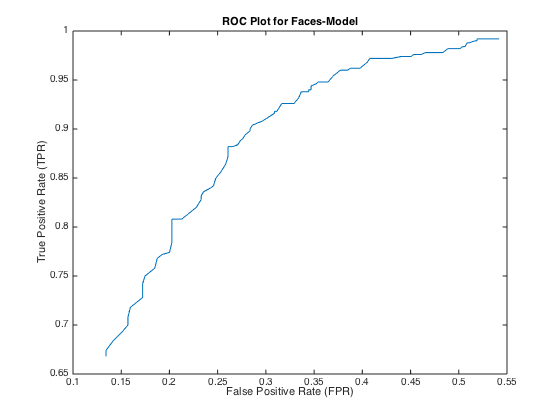
\includegraphics[scale=0.6]{plot_roc_face}
\subsubsection{ROC curve usinf non face model as predictor}
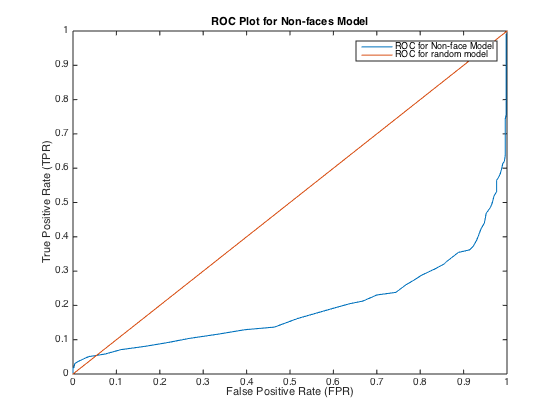
\includegraphics[scale=0.6]{plot_roc_non_face}
\subsection{Threshold for FPR $\leq$ 0.2}
We find that the loglikelihood score threshold for the faces model is 40 and for the non faces model is 24 such that FPR $\leq$ 0.2
\section{Inferences}
\subsection{Suitable model for classification task}
By performing this experiment, we realise that using the faces model is better suited than using the non faces model for classification tasks because the ROC curve for faces model is always above the ROC curve for non-faces model. Also we notice that the ROC curve for the non-faces model is below the $y=x$ line which is essentially the ROC curve we get by randomly classifying the images as either face or non face. Hence the non-face model performs worse than a random classifier.
\newline
Also, intuitively speaking using the faces-model as a classifier also makes sense because faces will have a lot of features common amongst themselves which is not the case with non-faces.

\end{document}
